%% LyX 1.3 created this file.  For more info, see http://www.lyx.org/.
%% Do not edit unless you really know what you are doing.
\documentclass[english, 12pt]{article}
\usepackage{times}
%\usepackage{algorithm2e}
\usepackage{url}
\usepackage{bbm}
\usepackage[T1]{fontenc}
\usepackage[latin1]{inputenc}
\usepackage{geometry}
\geometry{verbose,letterpaper,tmargin=2.5cm,bmargin=2.5cm,lmargin=2.5cm,rmargin=2.5cm}
\usepackage{rotating}
\usepackage{graphicx}
\usepackage{amsmath, amsthm, amssymb}
\usepackage{setspace}
\usepackage{lineno}
\usepackage{hyperref}
\usepackage{bbm}

%\usepackage{xcolor,framed}
%\colorlet{shadecolor}{blue!10}
%\begin{shaded}blabla\end{shaded}


%\usepackage{xr}
%\externaldocument{PRS-supp}

\linenumbers
\doublespacing
%\usepackage[authoryear]{natbib}
\usepackage{natbib} \bibpunct{(}{)}{;}{author-year}{}{,}

%Pour les rajouts
\usepackage{xcolor}

\usepackage{dsfont}
\usepackage[warn]{textcomp}
\usepackage{adjustbox}
\usepackage{multirow}
\usepackage{graphicx}
\graphicspath{{figures/}}
\DeclareMathOperator*{\argmin}{\arg\!\min}

\let\tabbeg\tabular
\let\tabend\endtabular
\renewenvironment{tabular}{\begin{adjustbox}{max width=\textwidth}\tabbeg}{\tabend\end{adjustbox}}

\makeatletter

%%%%%%%%%%%%%%%%%%%%%%%%%%%%%% LyX specific LaTeX commands.
%% Bold symbol macro for standard LaTeX users
%\newcommand{\boldsymbol}[1]{\mbox{\boldmath $#1$}}

%% Because html converters don't know tabularnewline
\providecommand{\tabularnewline}{\\}
\definecolor{clumping}{HTML}{38761D}
\definecolor{thresholding}{HTML}{1515FF}
%<span style="color:#38761D">Clumping</span> + <span style="color:#1515FF">Thresholding</span>

\usepackage{babel}
\makeatother


\begin{document}

\section{Introduction}

In my thesis work, we have been focusing on assessing someone's risk of disease based on DNA mutations data. DNA mutations do not really change over lifetime so that we could, in theory, assess someone's risk of disease at birth. Thus, this could have potentially large implications in disease prevention. As an example, about 12\% of women in the general population will develop breast cancer sometime during their lives \cite[]{desantis2016breast}. By contrast, a recent large study estimated that about 72\% (95\% CI: 65\%-79\%) of women who inherit a harmful BRCA1 mutation and about 69\% (95\% CI: 61\%-77\%) of women who inherit a harmful BRCA2 mutation will develop breast cancer by the age of 80 \cite[]{kuchenbaecker2017risks}. In 2013, Angelina Jolie announced that she had undergone a preventative double mastectomy, because she had a family history of breast cancer and was carrying a harmful BRCA1 mutation.

In this introduction, [TODO]

\subsection{[SOMEWHERE?]}

Selection might also be responsible for keeping genetic effect sizes low, since variants of larger effect may be selected against and eventually disappear \cite[]{pritchard2002allelic}.

\subsection{Context}

Today, clinical risk prediction for common adult-onset diseases often relies on basic demographic characteristics, such as age, gender and ethnicity; basic health parameters and lifestyle factors, such as body mass index, smoking status, alcohol consumption and physical exercise habits; measurement of clinical risk factors proximal to overt disease onset, such as blood pressure levels, blood chemistries or biomarkers indicative of ongoing disease processes; ascertainment of environmental exposures, such as air pollution, heavy metals and other environmental toxins; and family history \cite[]{torkamani2018personal}.
Routine genetic profiling is conspicuously absent from this list, often relegated to use only when testing clarifies individual-level risks in the context of a known family history for some common adult-onset
diseases \cite[]{torkamani2018personal}.

\subsubsection{Different types of disease and mutations}

Different types of mutations exist (Figure \ref{fig:rare-common}).
[PARLER DE DISEASE ARCHITECTURE??]
Along with harmful BRCA mutations, many other highly penetrant mutations\footnote{most people carrying the mutation will develop the disease} are associated with diseases, and are searchable in an online database \cite[]{hamosh2005online}. Those mutation are often very rare and are either associated with some very rare disease or are explaining only a small proportion of common disease incidence.
In this work, we focus on common diseases (e.g.\ breast cancer) and try to predict individuals' disease susceptibility based on common variants; the common disease--common variant hypothesis \cite[]{pritchard2002allelic}. This hypothesis further suggests that such diseases are likely caused by a large number of common variants, each contributing only a small risk and thereby evading negative evolutionary selection \cite[]{salari2012personalized}.
One common form of variation across human genomes is called a single nucleotide polymorphism (SNP). As indicated by the name, SNPs are single base changes in the DNA.
Sequencing technologies now exists to genotype hundreds of thousands of variants at once for around \$50 only. Starting with the \cite{wellcome2007genome}, these new sequencing technologies had led to many genome-wide association studies.%, which we talk about in the next section. From these studies, it was found that effects of common variants that are associated with some disease are typically very small.

\begin{figure}[htb]
\centerline{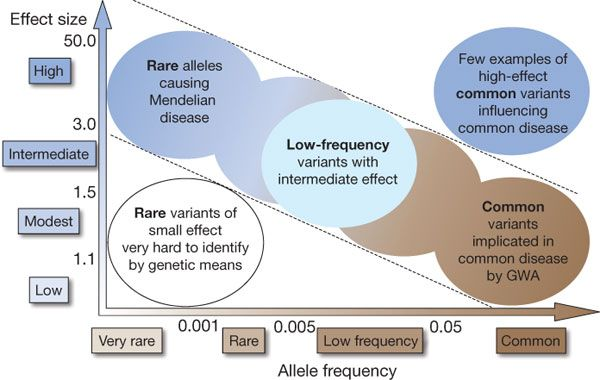
\includegraphics[width=0.7\textwidth]{rare-common.jpg}}
\caption{Feasibility of identifying genetic variants by risk allele frequency and strength of genetic effect (odds ratio). Most emphasis and interest lies
in identifying associations with characteristics shown within diagonal dotted
lines. Source: \cite{manolio2009finding}.}
\label{fig:rare-common}
\end{figure}

\subsubsection{Genome-Wide Association Studies (GWAS)}

\cite{visscher201710} provide a thorough review of the aims and outcomes of GWAS.
The method behind GWAS is simple: test each variant one by one for association with a phenotype of interest.
For a continuous phenotype (e.g.\ height), linear regression is used and a t-test is performed on $\beta^{(j)}$ for each SNP $j$ where
\begin{equation}
\hat{y} = \alpha^{(j)} + \beta^{(j)} SNP^{(j)} + \gamma_1^{(j)} COV_1 + \cdots + \gamma_K^{(j)} COV_K + \epsilon~,\label{eq:gwas1}
\end{equation}
$K$ is the number of covariates, including principal components and other covariates such as age and gender. Similarly, for a binary phenotype (e.g.\ disease status), logistic regression is used and a Z-test is performed on $\beta^{(j)}$ for each SNP $j$ where
\begin{equation}
\log{\left(\frac{\hat{p}}{1-\hat{p}}\right)} = \alpha^{(j)} + \beta^{(j)} SNP^{(j)} + \gamma_1^{(j)} COV_1 + \cdots + \gamma_K^{(j)} COV_K + \epsilon~,\label{eq:gwas2}
\end{equation}
$\hat{p} = \mathbb{P}(Y = 1)$ and $Y$ denotes the binary phenotype.
It is well established that principal components of genotype data should be included as covariates in GWAS \cite[]{price2006principal}. Indeed, principal components of genotype data capture well population structure (as shown in figure \ref{fig:pca}). 
For example, consider a dataset where you have 900 Finnish people and only 100 Italian people. Because Finnish people are taller than Italian people, any SNP with a large difference in allele frequency between these two populations would be flagged as being associated with height, leading to many false positive associations. Adding principal components as covariates aims at preventing those SNPs from being false positive reports [PARLER DE QQ-PLOT ET DE LAMBDAGC??].

\begin{figure}[htb]
\centerline{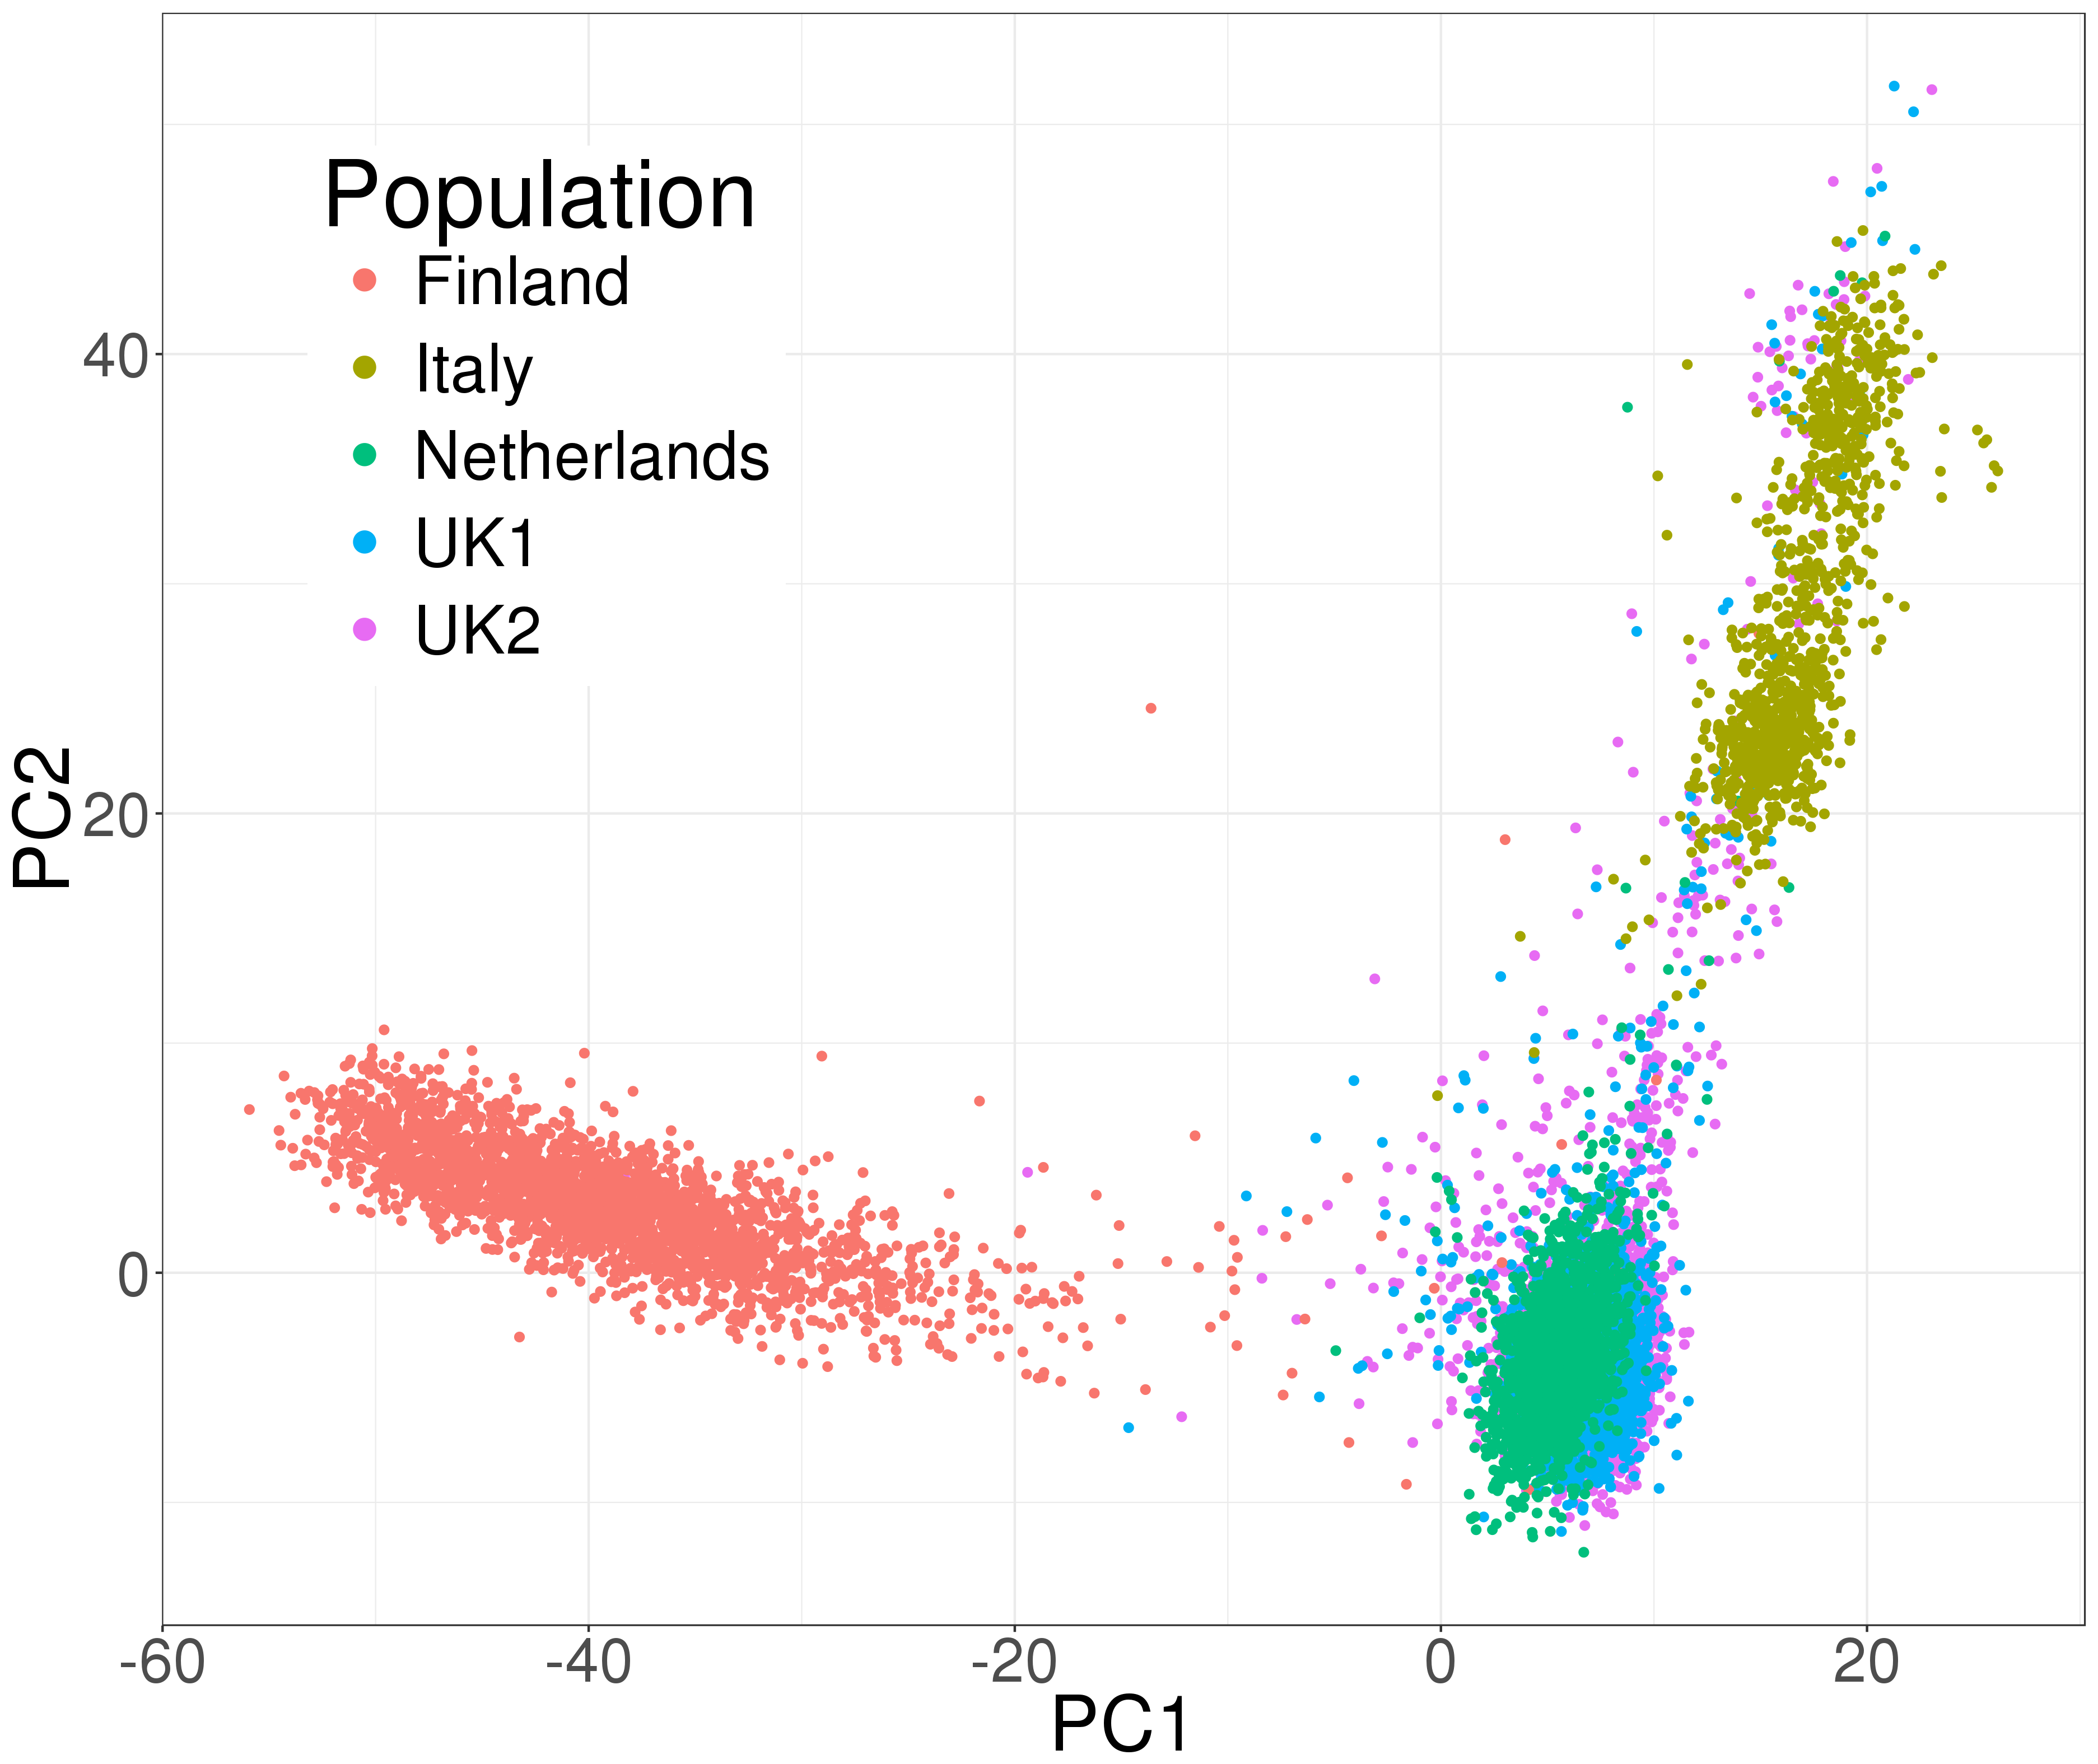
\includegraphics[width=0.6\textwidth]{celiac-pca.png}}
\caption{First two Principal Components of individuals from four European populations. PC1 correlates with latitude while PC2 correlates longitude.}\label{fig:pca}
\end{figure}

These simple tests can be used only if individuals are not related to one another. If they do, a common practice is to remove one individual from each pairs of related individuals. Another strategy is to use Linear Mixel Models (LMM) to take into account both relatedness and population structure; these mixed models have also the potential to increase discovery power \cite[]{yang2014advantages}.

To date, more than 10,000 strong associations have been reported between genetic variants and one or more complex traits \cite[]{welter2013nhgri}, where ``strong'' is defined as statistically significant at the genome-wide p-value threshold of $5 \cdot 10^{-8}$, which corresponds to a type-I error of 5\%, Bonferroni-corrected for one million independent tests \cite[]{pe2008estimation}. Results of a GWAS are usually reported in a Manhattan plot (Figure \ref{fig:gwas}). This type of plot shows some association peaks (similar to skyscrapers in Manhattan) due to some local correlation between SNPs (Linkage Disequilibrium), with squared correlation roughly inversely proportional to distance between SNPs \cite[]{hudson2001two}.

\begin{figure}[htb]
\centerline{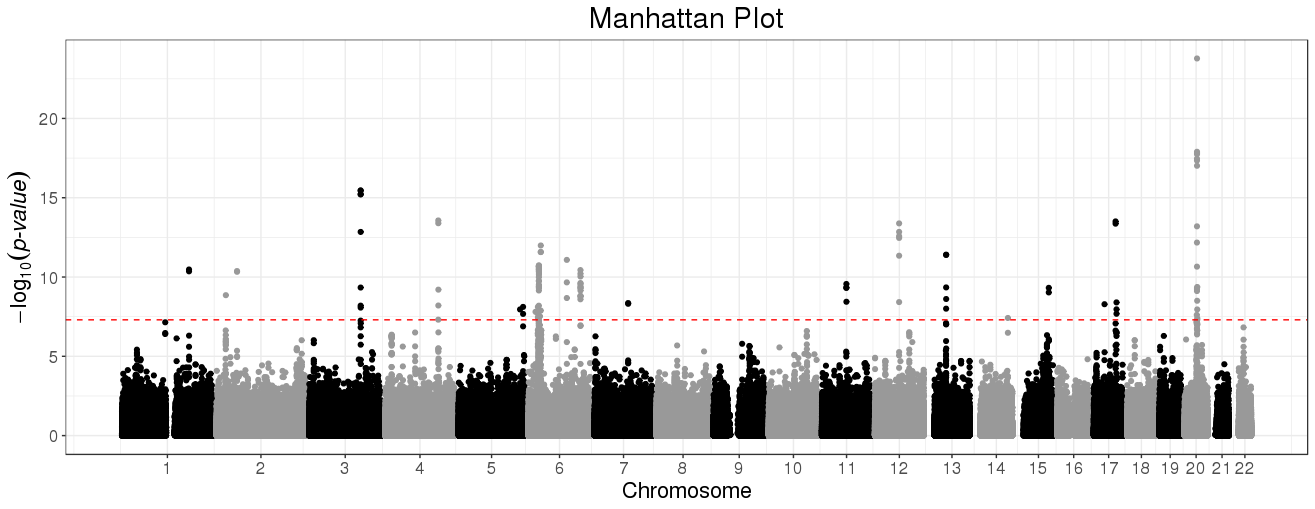
\includegraphics[width=0.95\textwidth]{gwas-height-20K.png}}
\caption{Manhattan plot of GWAS of height based on 20,000 unrelated individuals.}\label{fig:gwas}
\end{figure}


\subsubsection{GWAS data}

There are mainly three types of data: genotyped SNPs from genotyping chips, imputed SNPs from reference panels and Next Generation Sequencing (NGS) data.
Genotyping chips enables a quick and cheap genotyping of 200K to 2M SNPs, mostly focusing on common variants (Minor Allele Frequency (MAF) larger than 5\%). From this genotyping, you can get a matrix of $0$s, $1$s and $2$s, counting the number of alternative alleles for each individual (row) and each genome position (column). There are usually few missing values (less than 5\% in total).

Imputation has a different meaning in genetics than in other Data Science fields; it does not refer to filling those 5\% missing values, but instead refers to adding completely new variants that were not genotyped with the chip used. 
Imputation is enabled by the fact that the genotypes of unobserved genetic variants can be predicted by the haplotypes inferred from multiple observed SNPs (the ones that were genotyped) and the haplotypes observed from a fully sequenced reference
panel \cite[]{marchini2010genotype,mccarthy2016reference}.
Imputation now allows to have datasets such as the UK Biobank: 90M SNPs for each of 500K individuals \cite[]{bycroft2017genome}.

Finally, NGS (also called Whole Genome Sequencing (WGS)) refers to fully sequenced data over more than 3M variants, including some rare variants. Yet, this technology is still very expensive, with a cost of around \$1000 per genome.
GWAS to date have been based on SNP arrays designed to tag common variants in the genome. These arrays do not cover all genetic variants in the population, and it seems natural that future GWAS will be based on WGS. However, the price differential between SNP arrays and WGS is still substantial, and array technology remains more robust than sequencing \cite[]{visscher201710}. An in-between solution could be to use extremely low-coverage sequencing \cite[]{pasaniuc2012extremely}.

Recently, some national biobanks projects have emerged. For example, the UK Biobank has released both genome-wide genotypes and rich phenotypic data on 500K individuals to the international research community \cite[]{bycroft2017genome}.
Yet, most of the time, only summary statistics for a GWAS dataset (estimated effect sizes and p-values of SNPs) are available (not the individual-level genotype data). Because of the availability of such data en masse, specific methods using those summary data have been developed \cite[]{pasaniuc2014fast,vilhjalmsson2015modeling,bulik2015ld,pasaniuc2017dissecting,speed2018sumher}. The craze for such data can be explained by the fact that GWAS individual-level data, sometimes consisting of a meta-analysis of many small datasets, cannot be easily shared publicly, as opposed to summary data. Moreover, methods using summary statistics data are usually fast and easy to use, making them even more appealing to researchers.

In this thesis, we used genotyped SNPs, imputed SNPs and summary statistics.


%%%%%%%%%%%%%%%%%%%%%%%%%%%%%%%%%%%%%%%%%%%%%%%%%%%%%%%%%%%%%%%%%%%%%%%%%%%%%%%%


\subsection{From GWAS to Polygenic Risk Scores (PRS)}

\subsubsection{A standard way to compute PRS}\label{sec:C+T}

The main method for computing Polygenic Risk Scores (PRS) is the widely used ``Clumping + Thresholding'' (C+T, also called ``Pruning + Thresholding'' in the literature) model based on univariate GWAS summary statistics as described in equations \eqref{eq:gwas1} and \eqref{eq:gwas2}.
Under the C+T model, a coefficient of regression is learned independently for each SNP along with a corresponding p-value (the GWAS part). The SNPs are first clumped (C) so that there remains only SNPs that are weakly correlated with each other ($S_\text{clumping}$). Thresholding (T) consists in removing SNPs that are under a certain level of significance (p-value threshold $p_T$ to be determined). A polygenic risk score is defined as the sum of allele counts of the remaining SNPs weighted by the corresponding regression coefficients \cite[]{purcell2009common,Dudbridge2013,Euesden2015},
\[\rm{PRS}_i = \sum_{\substack{j \in S_\text{clumping} \\ p_j~<~p_T}} \hat\beta_j \cdot G_{i,j}~,\] where $\hat\beta_j$ ($p_j$) are the effect sizes (p-values) learned from the GWAS and $G_{i,j}$ is the allele count (genotype) for individual $i$ and SNP $j$.

\begin{figure}[htb]
\centerline{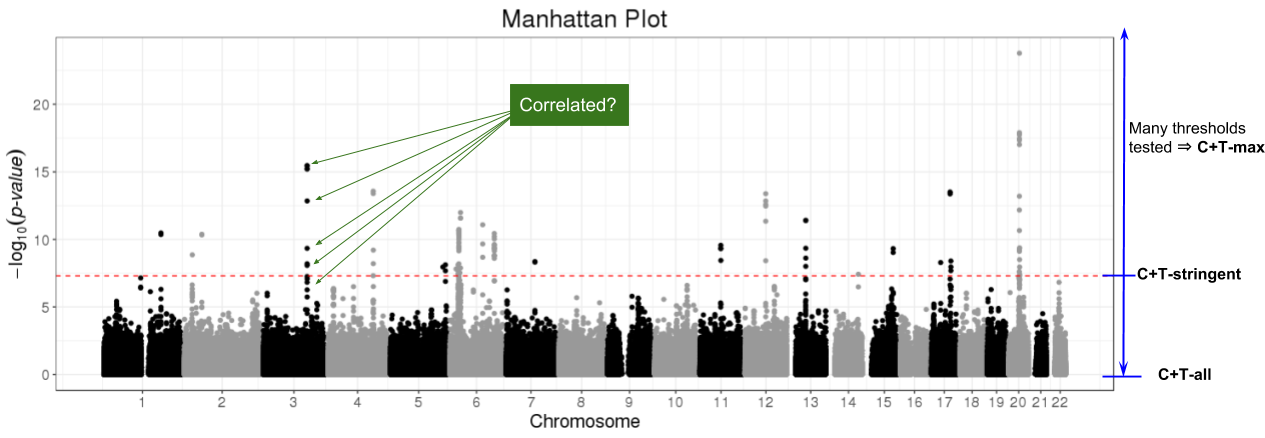
\includegraphics[width=0.95\textwidth]{GWAS2PRS3.png}}
\caption{Illustration of C+T looking at a Manhattan plot of GWAS of height based on 20,000 unrelated individuals. \textbf{\color{clumping}Clumping:} due to Linkage Disequilibrium, indirect associations provides only redundant information (see Figure \ref{fig:gwasLD}). \textbf{\color{thresholding}Thresholding:} SNPs are included in the polygenic score if they are significant enough in order to reduce noice in the score. [TODO: refaire]}\label{fig:gwas2}
\end{figure}

\begin{figure}[htb]
\centerline{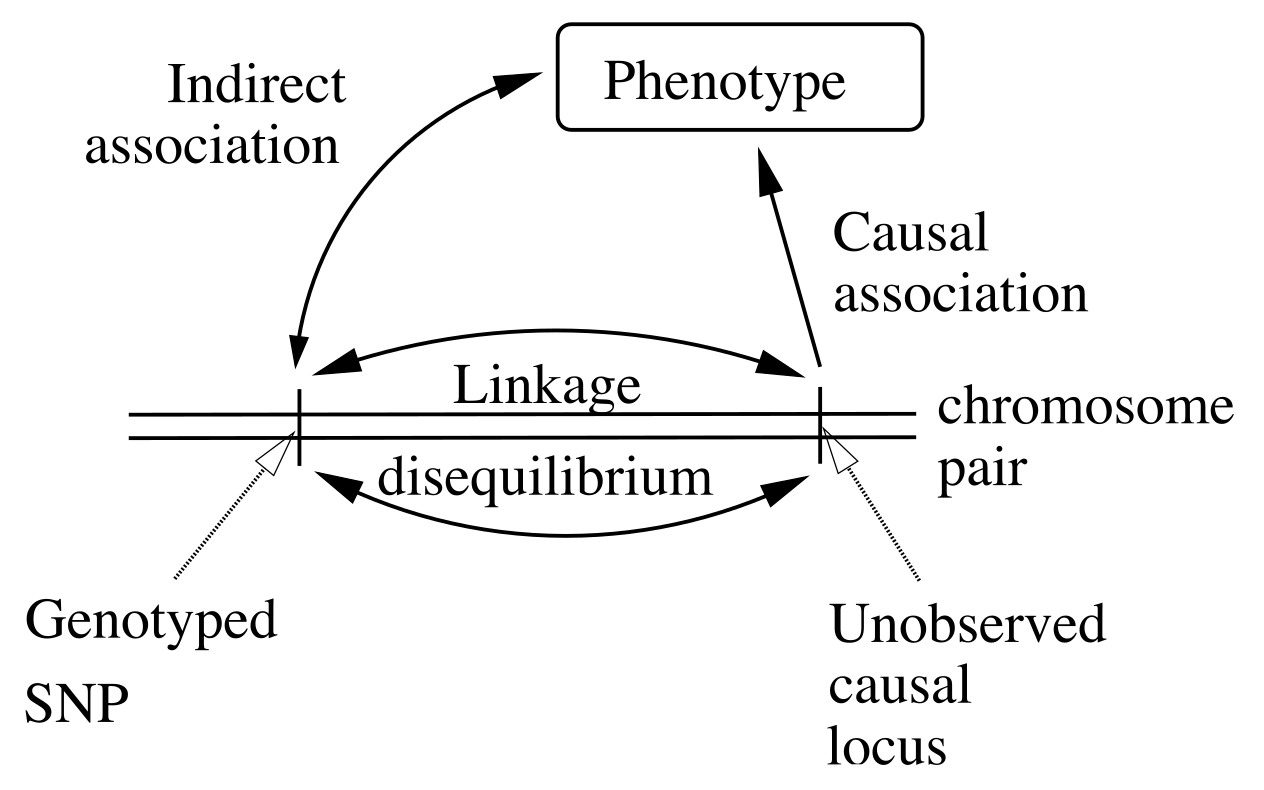
\includegraphics[width=0.5\textwidth]{indirect-association.png}}
\caption{Illustration of an indirect association with a phenotype due to Linkage Disequilibrium between SNPs. Source: \cite{astle2009population}.}\label{fig:gwasLD}
\end{figure}

\subsubsection{PRS for epidemiology}

Polygenic Risk Scores (PRS) have been used for epidemiology before being used for prediction. The steps for a PRS analysis are illustrated in figure \ref{fig:steps-PRS} and have two goals. First, PRS can be used when there is no SNP detected in a GWAS in order to show that there is still a significant polygenic contribution to the phenotype of intereset. 
For example, in 2009, a GWAS for Schizophrenia by \cite{purcell2009common} found only a single significantly associated SNP, although this disease is highly heritable. Yet, by constructing a PRS and testing it for association with Schizophrenia in another independent dataset, they proved that there is a polygenic contribution to Schizophrenia (Figure \ref{fig:epi-PRS}). 
Thus, polygenic analysis methods were central in demonstrating that the first phase of GWAS were underpowered, which propelled the drive for larger sample sizes that is now starting to pay off \cite[]{wray2014research}.

\begin{figure}[htb]
\centerline{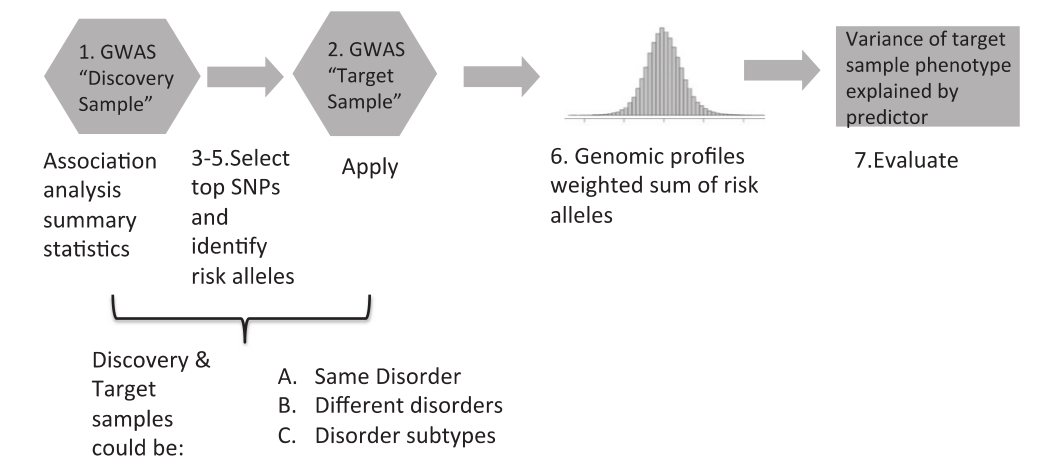
\includegraphics[width=0.8\textwidth]{genomic-profile.png}}
\caption{Illustration of the steps in genomic profile risk scoring. Source: \cite{wray2014research}.}\label{fig:steps-PRS}
\end{figure}

\begin{figure}[htb]
\centerline{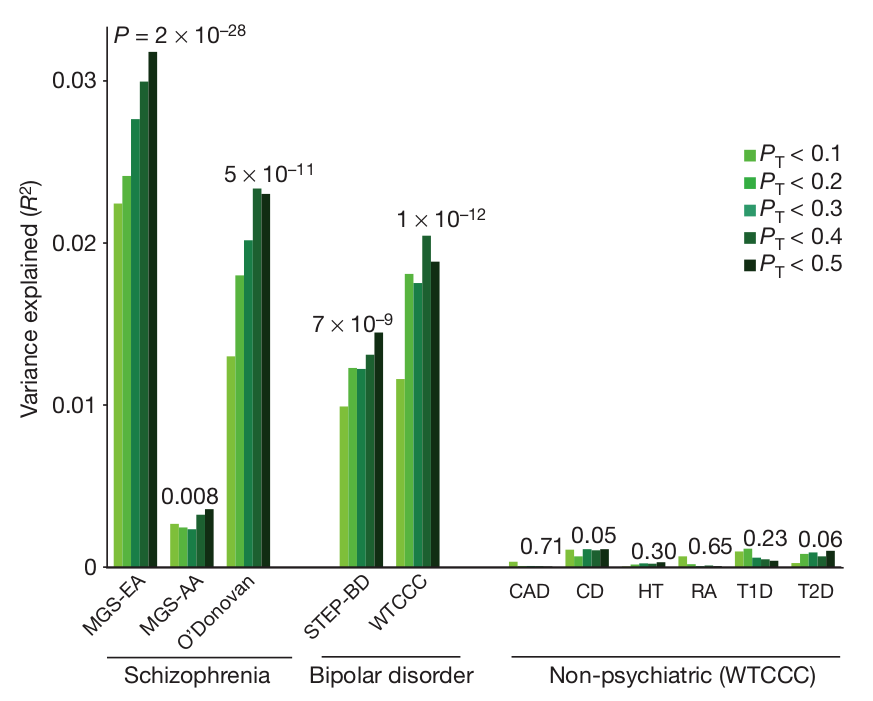
\includegraphics[width=0.65\textwidth]{purcell2009.png}}
\caption{Replication of the polygenic component derived by the International Schizophrenia Consortium in independent schizophrenia and bipolar disorder samples. Source: \cite{purcell2009common}.}\label{fig:epi-PRS}
\end{figure}

Another use of PRS for epidemiology is to test the PRS for association with a phenotype that is different from the one used to construct the PRS.
This technique enables researchers to prove that there is a common genetic contribution between two traits. 
For example, it was shown that there is a common genetic contribution between Schizophrenia and bipolar disorder (Figure \ref{fig:epi-PRS}). 


\subsubsection{The differing goals of association testing and risk prediction}

Association testing (GWAS) and prediction have very different goals.
First, GWAS aims at identifying highly replicable disease-associated variants by using a highly stringent p-value threshold to prevent false discoveries. However, using only hits from GWAS results in PRS of low predictive value (see section \ref{sec:missing}). 
A common mistake is to report highly significant findings with large odds ratios as useful predictors of disease. 
Thus, many people have reminded researchers over the years that GWAS findings are not predictive on their own, and that we would need scores that combine many SNPs in order to have a decent predictor of disease, i.e. polygenic scores \cite[]{pepe2004limitations,janssens2006predictive,jakobsdottir2009interpretation,wald2019illusion}.
Finally, it should be noted that population stratification, usually considered an unwelcome confounder in GWAS, may be useful in risk prediction and may be leveraged to produce better models \cite{golan2014effective,abraham2015genomic}.

[AJOUTER DES CHOSES DE ABRAHAM 2015??]


\subsection{Genomic prediction}

\subsubsection{Heritability and missing heritability} \label{sec:missing}

The basic components of disease risk are usually broken down into genetic susceptibility, environmental exposures and lifestyle factors. Thus, all disease incidence cannot be predicted by genetic factors only.
For a quantitative phenotype, we call heritability ($h^2$) the proportion of phenotypic variation that is attributable to genetic factors \cite[]{visscher2008heritability}.
Methods now enable the estimation of chip-heritability (also called SNP-heritability: $h^2_{SNP}$) using linear mixed models and residual maximum likelihood. For example, for a chip of 300K SNPs, it was shown that those SNPs could account for 45\% of the variance of height \cite[]{yang2010common}.
Note that the heritability of height is estimated to be around 80\% \cite[]{silventoinen2003determinants,visscher2006assumption}; the difference between these two values can be explained by the fact that 300K SNPs cannot capture the same variation in height as the 3 billion base pairs of DNA. This difference can also reflect an overestimation of heritability.

So, basically, heritability is the upper bound in terms of prediction power (when measured with $R^2$) that we can get using a model from genetic variants only.
The difference between $R^2$ and $h^2$ has been termed ``missing heritability'' \cite[]{manolio2009finding}. So, the main goal of genomic prediction and my thesis is to get best possible predictions based on genetic data in order to reduce this missing heritability.

First GWAS found only 12 associated SNPs for type 2 diabetes and only 2 for protaste cancer, explaining a small part of heritability of these diseases \cite[]{jakobsdottir2009interpretation}. Likewise, in 2008, only 40 genome-wide-significant SNPs had been identified for height, and together these explained about 5\% of heritability \cite[]{manolio2009finding}. In 2014, the number of associated SNPs had increased to around 700, explaining 20\% of heritability \cite[]{wood2014defining}.
Since most of the identified associated SNPs have effect size close to the limit dictated by the power of the studies, a likely explanation, at least in part, is that there are many common polymorphisms with effects that were too small to pass the stringent significance thresholds \cite[]{wray2008prediction}.
Therefore, as results from multiple GWAS are combined, a larger fraction of the genetic variance is likely to be explained and accurate prediction of genetic risk to disease will become possible even though the risks conveyed by individual variants are small \cite[]{wray2008prediction}.
%Therefore, sample size is not large enough to detect and estimate SNP effects precisely enough, but we can hope that with increasing sample sizes, more variants will be detected and more heritability could be explained by genetic variants.


\subsubsection{Methods for genomic prediction}

Several methods have been developed to predict disease status based on SNP information.
We can divide these methods in two categories: the ones that use summary statistics and the ones that use individual-level data only.
The most widely used methods called ``Clumping + Thresholding'' (C+T) has been described in section \ref{sec:C+T}.
Later, two other techniques have been developed that focus on using correlation structure of a reference panel to account for LD, instead of discarding SNPs in LD through clumping \cite{vilhjalmsson2015modeling,mak2017polygenic}. 
[ADD OTHER BIORXIV PAPERS?? NPS/PRS-CS?]

When using individual-level data only, the problem boils down to a statistical learning classification problem. Thus, some statistical learning methods have been used to derive PRS for complex human diseases by jointly estimating SNP effects. Such methods include joint logistic regression, Support Vector Machine (SVM) and random forests \cite[]{wei2009disease,abraham2012sparsnp,abraham2014accurate,botta2014exploiting,okser2014regularized}.
Linear Mixed-Models (LMMs) are another widely-used method in fields such as plant and animal breeding or for predicting highly heritable quantitative human phenotypes such as height \cite[]{yang2010common}. 
However, these methods and their derivatives are often computationally very demanding, both in terms of memory and time required \cite[]{zhou2013polygenic,golan2014effective,speed2014multiblup,maier2015joint}.
Recently, two methods primarily designed for association testing, BOLT-LMM and SAIGE, have been developed to handle very large datasets \cite[]{loh2018mixed,zhou2018efficiently}.

\subsubsection{Objective and main difficulties of the thesis}


\newpage

\bibliographystyle{natbib}
\bibliography{refs}

\end{document}
